\section{What we are working on}

\begin{frame}{Further inductance characterization}

    Even if maybe not relevant for control purposes, we are trying to \textbf{study the dependence of the inductance on both the ball position and the current}.
    \begin{equation}
        L = L(z, I) = L_0 + L_z e^{-a_z z} + L_I \tanh(-a_I I)
    \end{equation}

    \begin{columns}[c, onlytextwidth]

        \begin{column}{0.65\textwidth}

            \begin{figure}
                \centering
                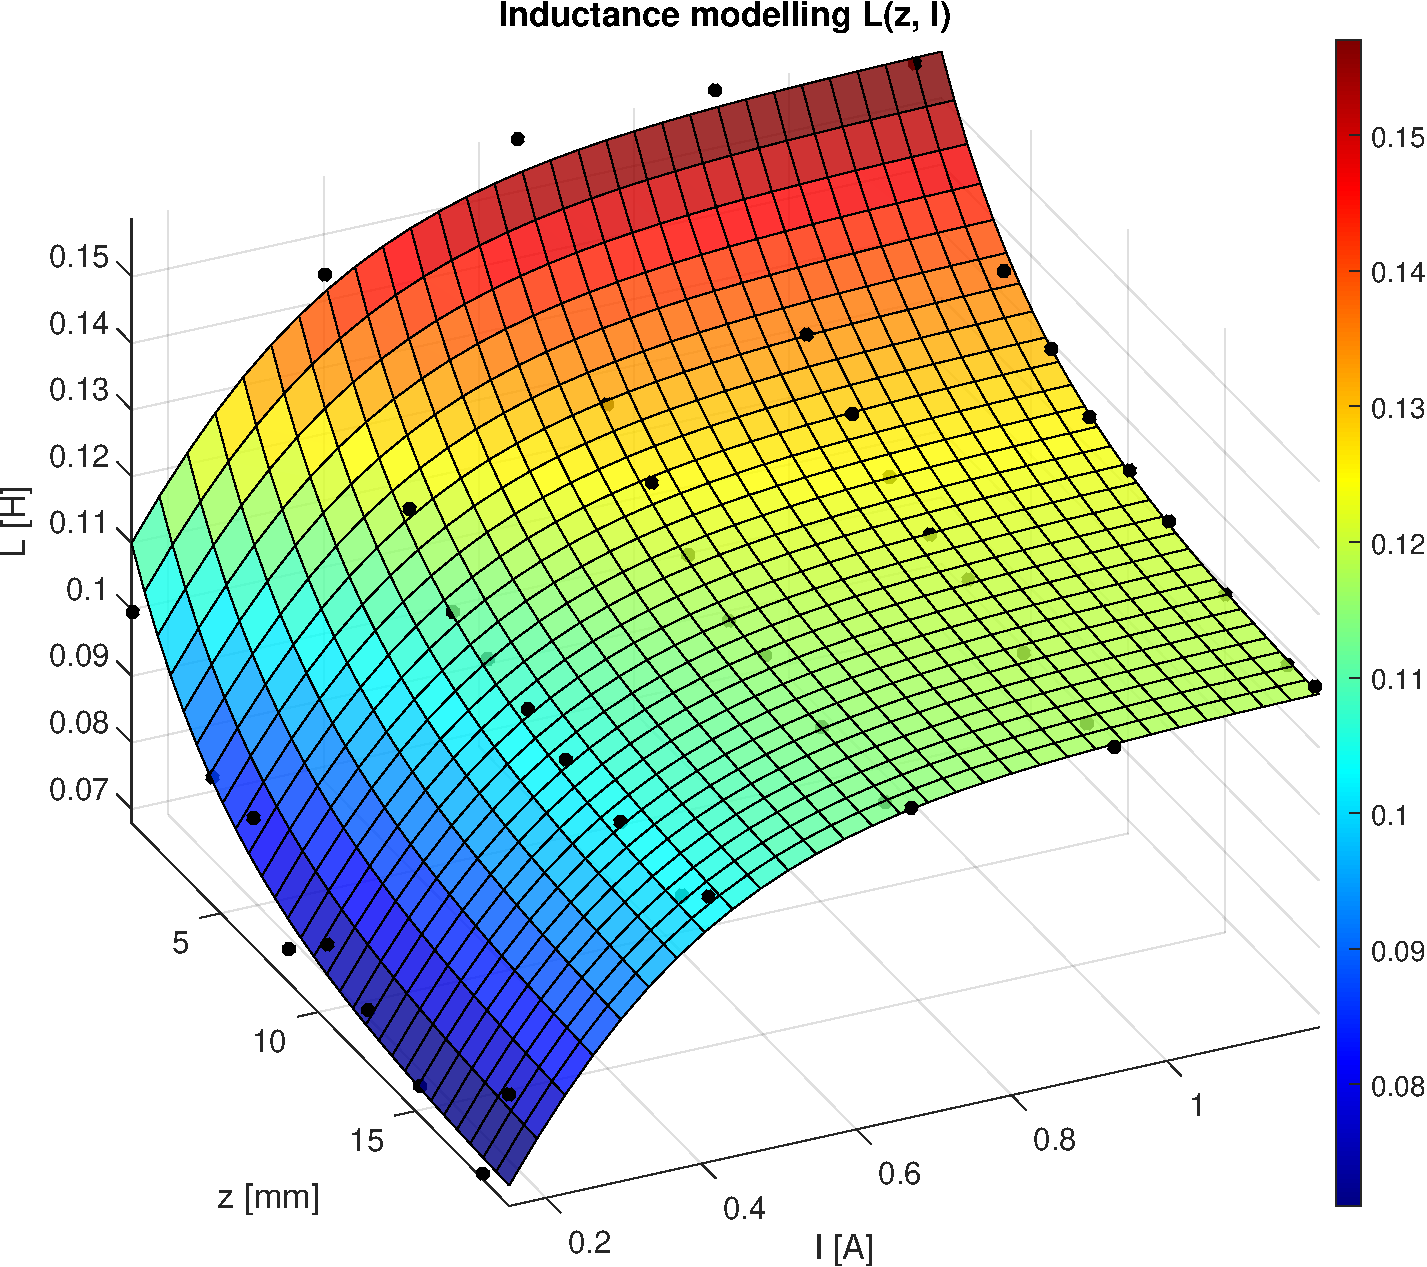
\includegraphics[width=0.8\textwidth]{img/MATLAB/measurements/inductance.pdf}
                \caption{Fitted model for $L(z, I)$}
            \end{figure}
        \end{column}

        \begin{column}{0.35\textwidth}

            Higher current values are needed to obtain experimental data over all the possible operating regions.

        \end{column}

    \end{columns}

\end{frame}



\begin{frame}{MCP controller}

    We are currently trying to implement a Model Predictive Controller (MPC).

    We want to switch from classical linearized restricted state-space controllers to a more advanced and robust controller.

    However, looks like Simulink doesn't really like the way we are doing it\dots many implementation issues.

\end{frame}